% Created by tikzDevice version 0.12 on 2019-07-24 15:29:02
% !TEX encoding = UTF-8 Unicode
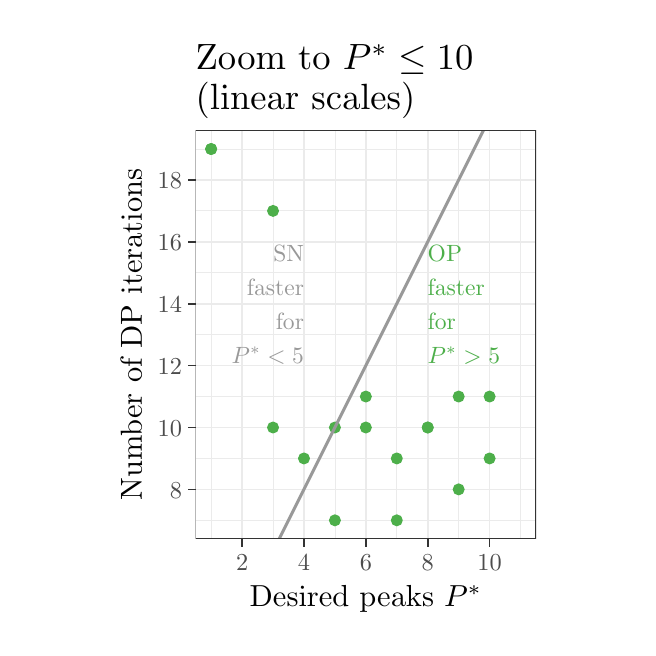
\begin{tikzpicture}[x=1pt,y=1pt]
\definecolor{fillColor}{RGB}{255,255,255}
\path[use as bounding box,fill=fillColor,fill opacity=0.00] (0,0) rectangle (216.81,216.81);
\begin{scope}
\path[clip] ( 27.61,  0.00) rectangle (189.20,216.81);
\definecolor{drawColor}{RGB}{255,255,255}
\definecolor{fillColor}{RGB}{255,255,255}

\path[draw=drawColor,line width= 0.6pt,line join=round,line cap=round,fill=fillColor] ( 27.61,  0.00) rectangle (189.20,216.81);
\end{scope}
\begin{scope}
\path[clip] ( 60.70, 32.08) rectangle (183.70,179.67);
\definecolor{fillColor}{RGB}{255,255,255}

\path[fill=fillColor] ( 60.70, 32.08) rectangle (183.70,179.67);
\definecolor{drawColor}{gray}{0.92}

\path[draw=drawColor,line width= 0.3pt,line join=round] ( 60.70, 38.79) --
	(183.70, 38.79);

\path[draw=drawColor,line width= 0.3pt,line join=round] ( 60.70, 61.15) --
	(183.70, 61.15);

\path[draw=drawColor,line width= 0.3pt,line join=round] ( 60.70, 83.52) --
	(183.70, 83.52);

\path[draw=drawColor,line width= 0.3pt,line join=round] ( 60.70,105.88) --
	(183.70,105.88);

\path[draw=drawColor,line width= 0.3pt,line join=round] ( 60.70,128.24) --
	(183.70,128.24);

\path[draw=drawColor,line width= 0.3pt,line join=round] ( 60.70,150.60) --
	(183.70,150.60);

\path[draw=drawColor,line width= 0.3pt,line join=round] ( 60.70,172.96) --
	(183.70,172.96);

\path[draw=drawColor,line width= 0.3pt,line join=round] ( 66.29, 32.08) --
	( 66.29,179.67);

\path[draw=drawColor,line width= 0.3pt,line join=round] ( 88.66, 32.08) --
	( 88.66,179.67);

\path[draw=drawColor,line width= 0.3pt,line join=round] (111.02, 32.08) --
	(111.02,179.67);

\path[draw=drawColor,line width= 0.3pt,line join=round] (133.38, 32.08) --
	(133.38,179.67);

\path[draw=drawColor,line width= 0.3pt,line join=round] (155.74, 32.08) --
	(155.74,179.67);

\path[draw=drawColor,line width= 0.3pt,line join=round] (178.11, 32.08) --
	(178.11,179.67);

\path[draw=drawColor,line width= 0.6pt,line join=round] ( 60.70, 49.97) --
	(183.70, 49.97);

\path[draw=drawColor,line width= 0.6pt,line join=round] ( 60.70, 72.33) --
	(183.70, 72.33);

\path[draw=drawColor,line width= 0.6pt,line join=round] ( 60.70, 94.70) --
	(183.70, 94.70);

\path[draw=drawColor,line width= 0.6pt,line join=round] ( 60.70,117.06) --
	(183.70,117.06);

\path[draw=drawColor,line width= 0.6pt,line join=round] ( 60.70,139.42) --
	(183.70,139.42);

\path[draw=drawColor,line width= 0.6pt,line join=round] ( 60.70,161.78) --
	(183.70,161.78);

\path[draw=drawColor,line width= 0.6pt,line join=round] ( 77.48, 32.08) --
	( 77.48,179.67);

\path[draw=drawColor,line width= 0.6pt,line join=round] ( 99.84, 32.08) --
	( 99.84,179.67);

\path[draw=drawColor,line width= 0.6pt,line join=round] (122.20, 32.08) --
	(122.20,179.67);

\path[draw=drawColor,line width= 0.6pt,line join=round] (144.56, 32.08) --
	(144.56,179.67);

\path[draw=drawColor,line width= 0.6pt,line join=round] (166.92, 32.08) --
	(166.92,179.67);
\definecolor{drawColor}{RGB}{77,175,74}
\definecolor{fillColor}{RGB}{77,175,74}

\path[draw=drawColor,line width= 0.4pt,line join=round,line cap=round,fill=fillColor] ( 66.29,172.96) circle (  1.96);

\path[draw=drawColor,line width= 0.4pt,line join=round,line cap=round,fill=fillColor] ( 88.66, 72.33) circle (  1.96);

\path[draw=drawColor,line width= 0.4pt,line join=round,line cap=round,fill=fillColor] ( 99.84, 61.15) circle (  1.96);

\path[draw=drawColor,line width= 0.4pt,line join=round,line cap=round,fill=fillColor] (111.02, 72.33) circle (  1.96);

\path[draw=drawColor,line width= 0.4pt,line join=round,line cap=round,fill=fillColor] (122.20, 83.52) circle (  1.96);

\path[draw=drawColor,line width= 0.4pt,line join=round,line cap=round,fill=fillColor] (133.38, 38.79) circle (  1.96);

\path[draw=drawColor,line width= 0.4pt,line join=round,line cap=round,fill=fillColor] (144.56, 72.33) circle (  1.96);

\path[draw=drawColor,line width= 0.4pt,line join=round,line cap=round,fill=fillColor] (155.74, 83.52) circle (  1.96);

\path[draw=drawColor,line width= 0.4pt,line join=round,line cap=round,fill=fillColor] (166.92, 61.15) circle (  1.96);

\path[draw=drawColor,line width= 0.4pt,line join=round,line cap=round,fill=fillColor] ( 66.29,172.96) circle (  1.96);

\path[draw=drawColor,line width= 0.4pt,line join=round,line cap=round,fill=fillColor] ( 88.66,150.60) circle (  1.96);

\path[draw=drawColor,line width= 0.4pt,line join=round,line cap=round,fill=fillColor] (111.02, 38.79) circle (  1.96);

\path[draw=drawColor,line width= 0.4pt,line join=round,line cap=round,fill=fillColor] (122.20, 72.33) circle (  1.96);

\path[draw=drawColor,line width= 0.4pt,line join=round,line cap=round,fill=fillColor] (133.38, 61.15) circle (  1.96);

\path[draw=drawColor,line width= 0.4pt,line join=round,line cap=round,fill=fillColor] (144.56, 72.33) circle (  1.96);

\path[draw=drawColor,line width= 0.4pt,line join=round,line cap=round,fill=fillColor] (155.74, 49.97) circle (  1.96);

\path[draw=drawColor,line width= 0.4pt,line join=round,line cap=round,fill=fillColor] (166.92, 83.52) circle (  1.96);
\definecolor{drawColor}{gray}{0.60}

\path[draw=drawColor,line width= 1.1pt,line join=round] ( 74.85,  0.00) -- (183.26,216.81);

\node[text=drawColor,anchor=base east,inner sep=0pt, outer sep=0pt, scale=  0.85] at ( 99.84,132.34) {SN};

\node[text=drawColor,anchor=base east,inner sep=0pt, outer sep=0pt, scale=  0.85] at ( 99.84,120.05) {faster};

\node[text=drawColor,anchor=base east,inner sep=0pt, outer sep=0pt, scale=  0.85] at ( 99.84,107.76) {for};

\node[text=drawColor,anchor=base east,inner sep=0pt, outer sep=0pt, scale=  0.85] at ( 99.84, 95.47) {$P^*<5$};
\definecolor{drawColor}{RGB}{77,175,74}

\node[text=drawColor,anchor=base west,inner sep=0pt, outer sep=0pt, scale=  0.85] at (144.56,132.34) {OP};

\node[text=drawColor,anchor=base west,inner sep=0pt, outer sep=0pt, scale=  0.85] at (144.56,120.05) {faster};

\node[text=drawColor,anchor=base west,inner sep=0pt, outer sep=0pt, scale=  0.85] at (144.56,107.76) {for};

\node[text=drawColor,anchor=base west,inner sep=0pt, outer sep=0pt, scale=  0.85] at (144.56, 95.47) {$P^*>5$};
\definecolor{drawColor}{gray}{0.20}

\path[draw=drawColor,line width= 0.6pt,line join=round,line cap=round] ( 60.70, 32.08) rectangle (183.70,179.67);
\end{scope}
\begin{scope}
\path[clip] (  0.00,  0.00) rectangle (216.81,216.81);
\definecolor{drawColor}{gray}{0.30}

\node[text=drawColor,anchor=base east,inner sep=0pt, outer sep=0pt, scale=  0.88] at ( 55.75, 46.72) {8};

\node[text=drawColor,anchor=base east,inner sep=0pt, outer sep=0pt, scale=  0.88] at ( 55.75, 69.08) {10};

\node[text=drawColor,anchor=base east,inner sep=0pt, outer sep=0pt, scale=  0.88] at ( 55.75, 91.45) {12};

\node[text=drawColor,anchor=base east,inner sep=0pt, outer sep=0pt, scale=  0.88] at ( 55.75,113.81) {14};

\node[text=drawColor,anchor=base east,inner sep=0pt, outer sep=0pt, scale=  0.88] at ( 55.75,136.17) {16};

\node[text=drawColor,anchor=base east,inner sep=0pt, outer sep=0pt, scale=  0.88] at ( 55.75,158.53) {18};
\end{scope}
\begin{scope}
\path[clip] (  0.00,  0.00) rectangle (216.81,216.81);
\definecolor{drawColor}{gray}{0.20}

\path[draw=drawColor,line width= 0.6pt,line join=round] ( 57.95, 49.97) --
	( 60.70, 49.97);

\path[draw=drawColor,line width= 0.6pt,line join=round] ( 57.95, 72.33) --
	( 60.70, 72.33);

\path[draw=drawColor,line width= 0.6pt,line join=round] ( 57.95, 94.70) --
	( 60.70, 94.70);

\path[draw=drawColor,line width= 0.6pt,line join=round] ( 57.95,117.06) --
	( 60.70,117.06);

\path[draw=drawColor,line width= 0.6pt,line join=round] ( 57.95,139.42) --
	( 60.70,139.42);

\path[draw=drawColor,line width= 0.6pt,line join=round] ( 57.95,161.78) --
	( 60.70,161.78);
\end{scope}
\begin{scope}
\path[clip] (  0.00,  0.00) rectangle (216.81,216.81);
\definecolor{drawColor}{gray}{0.20}

\path[draw=drawColor,line width= 0.6pt,line join=round] ( 77.48, 29.33) --
	( 77.48, 32.08);

\path[draw=drawColor,line width= 0.6pt,line join=round] ( 99.84, 29.33) --
	( 99.84, 32.08);

\path[draw=drawColor,line width= 0.6pt,line join=round] (122.20, 29.33) --
	(122.20, 32.08);

\path[draw=drawColor,line width= 0.6pt,line join=round] (144.56, 29.33) --
	(144.56, 32.08);

\path[draw=drawColor,line width= 0.6pt,line join=round] (166.92, 29.33) --
	(166.92, 32.08);
\end{scope}
\begin{scope}
\path[clip] (  0.00,  0.00) rectangle (216.81,216.81);
\definecolor{drawColor}{gray}{0.30}

\node[text=drawColor,anchor=base,inner sep=0pt, outer sep=0pt, scale=  0.88] at ( 77.48, 20.63) {2};

\node[text=drawColor,anchor=base,inner sep=0pt, outer sep=0pt, scale=  0.88] at ( 99.84, 20.63) {4};

\node[text=drawColor,anchor=base,inner sep=0pt, outer sep=0pt, scale=  0.88] at (122.20, 20.63) {6};

\node[text=drawColor,anchor=base,inner sep=0pt, outer sep=0pt, scale=  0.88] at (144.56, 20.63) {8};

\node[text=drawColor,anchor=base,inner sep=0pt, outer sep=0pt, scale=  0.88] at (166.92, 20.63) {10};
\end{scope}
\begin{scope}
\path[clip] (  0.00,  0.00) rectangle (216.81,216.81);
\definecolor{drawColor}{RGB}{0,0,0}

\node[text=drawColor,anchor=base,inner sep=0pt, outer sep=0pt, scale=  1.10] at (122.20,  7.62) {Desired peaks $P^*$};
\end{scope}
\begin{scope}
\path[clip] (  0.00,  0.00) rectangle (216.81,216.81);
\definecolor{drawColor}{RGB}{0,0,0}

\node[text=drawColor,rotate= 90.00,anchor=base,inner sep=0pt, outer sep=0pt, scale=  1.10] at ( 41.24,105.88) {Number of DP iterations};
\end{scope}
\begin{scope}
\path[clip] (  0.00,  0.00) rectangle (216.81,216.81);
\definecolor{drawColor}{RGB}{0,0,0}

\node[text=drawColor,anchor=base west,inner sep=0pt, outer sep=0pt, scale=  1.32] at ( 60.70,201.55) {Zoom to $P^* \leq 10$};

\node[text=drawColor,anchor=base west,inner sep=0pt, outer sep=0pt, scale=  1.32] at ( 60.70,187.30) {(linear scales)};
\end{scope}
\end{tikzpicture}
